\documentclass[border=4pt]{standalone}
\usepackage{tikz}
\usepackage{pgfplots}
\pgfplotsset{compat=1.18}
\usetikzlibrary{shapes.geometric,arrows.meta,positioning,calc,fit,decorations.pathreplacing,backgrounds}
\definecolor{boxblue}{RGB}{225,238,252}
\definecolor{boxgreen}{RGB}{225,247,231}
\definecolor{boxorange}{RGB}{253,236,216}
\definecolor{boxgray}{RGB}{237,237,237}
\definecolor{boxred}{RGB}{253,226,226}
\begin{document}
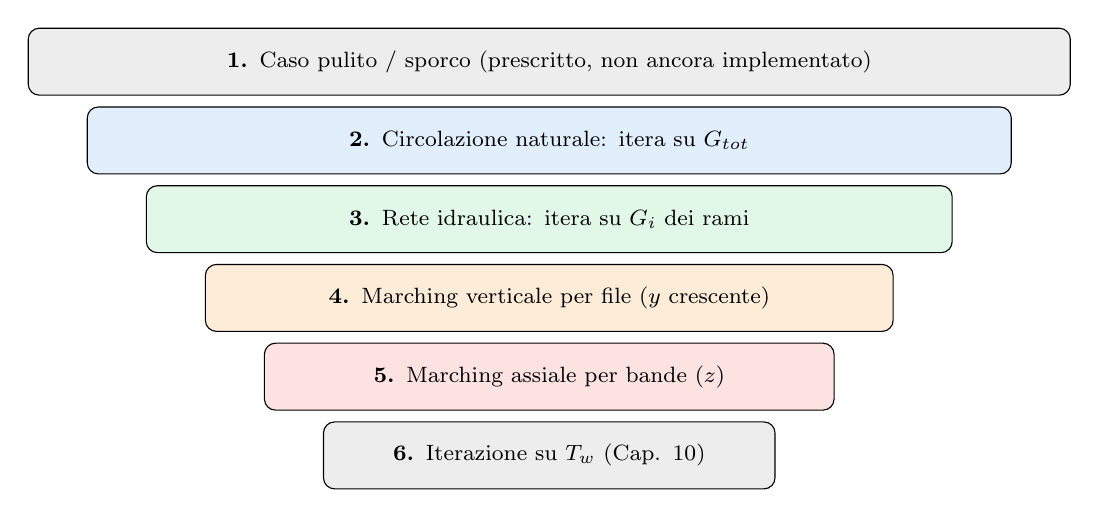
\begin{tikzpicture}[
  lvl/.style={draw, rectangle, rounded corners, align=center, font=\footnotesize, minimum height=0.85cm},
]
\node[lvl, fill=boxgray, text width=13cm] (l1) at (0,0) {\textbf{1.} Caso pulito / sporco (prescritto, non ancora implementato)};
\node[lvl, fill=boxblue, text width=11.5cm] (l2) at (0,-1.0) {\textbf{2.} Circolazione naturale: itera su $G_{tot}$};
\node[lvl, fill=boxgreen, text width=10cm] (l3) at (0,-2.0) {\textbf{3.} Rete idraulica: itera su $G_i$ dei rami};
\node[lvl, fill=boxorange, text width=8.5cm] (l4) at (0,-3.0) {\textbf{4.} Marching verticale per file ($y$ crescente)};
\node[lvl, fill=boxred, text width=7cm] (l5) at (0,-4.0) {\textbf{5.} Marching assiale per bande ($z$)};
\node[lvl, fill=boxgray, text width=5.5cm] (l6) at (0,-5.0) {\textbf{6.} Iterazione su $T_w$ (Cap. 10)};
\end{tikzpicture}
\end{document}
